\documentclass{standalone}

\usepackage{tikz}
\usetikzlibrary{arrows}
\usetikzlibrary{decorations.markings}
\usetikzlibrary{calc}

\begin{document}

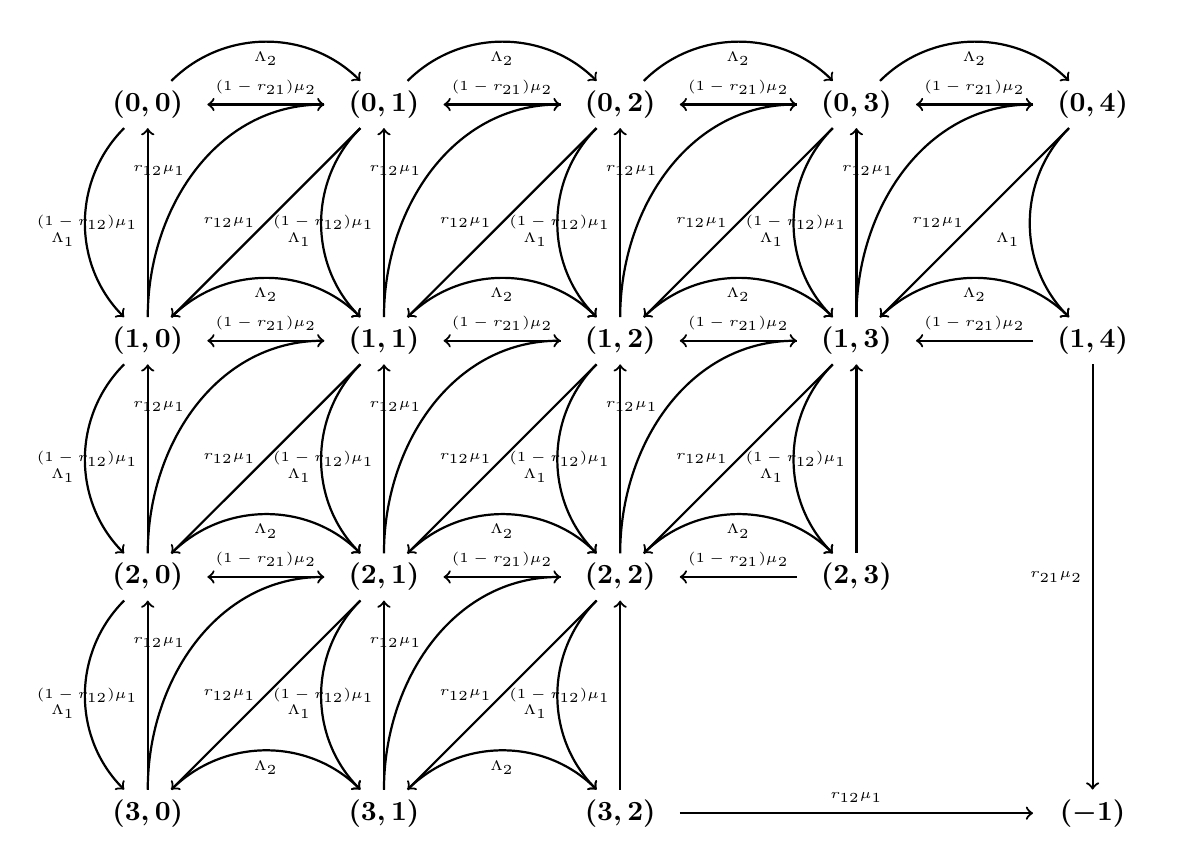
\begin{tikzpicture}
    \tikzstyle{state}=[minimum width=1.5cm, font=\boldmath];
    % First row
    \node (00) at (0,0) [state] {$(0,0)$};
    \node (01) at ($(00)+(3,0)$) [state] {$(0,1)$};
    \node (02) at ($(01)+(3,0)$) [state] {$(0,2)$};
    \node (03) at ($(02)+(3,0)$) [state] {$(0,3)$};
    \node (04) at ($(03)+(3,0)$) [state] {$(0,4)$};

    % Second row
    \node (10) at ($(00)+(0,-3)$) [state] {$(1,0)$};
    \node (11) at ($(10)+(3,0)$) [state] {$(1,1)$};
    \node (12) at ($(11)+(3,0)$) [state] {$(1,2)$};
    \node (13) at ($(12)+(3,0)$) [state] {$(1,3)$};
    \node (14) at ($(13)+(3,0)$) [state] {$(1,4)$};

    % Third row
    \node (20) at ($(10)+(0,-3)$) [state] {$(2,0)$};
    \node (21) at ($(20)+(3,0)$) [state] {$(2,1)$};
    \node (22) at ($(21)+(3,0)$) [state] {$(2,2)$};
    \node (23) at ($(22)+(3,0)$) [state] {$(2,3)$};

    % Fourth row
    \node (30) at ($(20)+(0,-3)$) [state] {$(3,0)$};
    \node (31) at ($(30)+(3,0)$) [state] {$(3,1)$};
    \node (32) at ($(31)+(3,0)$) [state] {$(3,2)$};

    \node (-1) at ($(32)+(6,0)$) [state] {$(-1)$};

    % Transitions
    % Arrivals
    \draw (00) edge[out=-135,in=135,->,thick] node [below left] {\tiny$\Lambda_1$} (10);
    \draw (01) edge[out=-135,in=135,->,thick] node [below left] {\tiny$\Lambda_1$} (11);
    \draw (02) edge[out=-135,in=135,->,thick] node [below left] {\tiny$\Lambda_1$} (12);
    \draw (03) edge[out=-135,in=135,->,thick] node [below left] {\tiny$\Lambda_1$} (13);
    \draw (04) edge[out=-135,in=135,->,thick] node [below left] {\tiny$\Lambda_1$} (14);

    \draw (10) edge[out=-135,in=135,->,thick] node [below left] {\tiny$\Lambda_1$} (20);
    \draw (11) edge[out=-135,in=135,->,thick] node [below left] {\tiny$\Lambda_1$} (21);
    \draw (12) edge[out=-135,in=135,->,thick] node [below left] {\tiny$\Lambda_1$} (22);
    \draw (13) edge[out=-135,in=135,->,thick] node [below left] {\tiny$\Lambda_1$} (23);

    \draw (20) edge[out=-135,in=135,->,thick] node [below left] {\tiny$\Lambda_1$} (30);
    \draw (21) edge[out=-135,in=135,->,thick] node [below left] {\tiny$\Lambda_1$} (31);
    \draw (22) edge[out=-135,in=135,->,thick] node [below left] {\tiny$\Lambda_1$} (32);

    \draw (00) edge[out=45,in=135,->,thick] node [below] {\tiny$\Lambda_2$} (01);
    \draw (01) edge[out=45,in=135,->,thick] node [below] {\tiny$\Lambda_2$} (02);
    \draw (02) edge[out=45,in=135,->,thick] node [below] {\tiny$\Lambda_2$} (03);
    \draw (03) edge[out=45,in=135,->,thick] node [below] {\tiny$\Lambda_2$} (04);

    \draw (10) edge[out=45,in=135,->,thick] node [below] {\tiny$\Lambda_2$}  (11);
    \draw (11) edge[out=45,in=135,->,thick] node [below] {\tiny$\Lambda_2$} (12);
    \draw (12) edge[out=45,in=135,->,thick] node [below] {\tiny$\Lambda_2$} (13);
    \draw (13) edge[out=45,in=135,->,thick] node [below] {\tiny$\Lambda_2$} (14);

    \draw (20) edge[out=45,in=135,->,thick] node [below] {\tiny$\Lambda_2$}  (21);
    \draw (21) edge[out=45,in=135,->,thick] node [below] {\tiny$\Lambda_2$} (22);
    \draw (22) edge[out=45,in=135,->,thick] node [below] {\tiny$\Lambda_2$} (23);

    \draw (30) edge[out=45,in=135,->,thick] node [below] {\tiny$\Lambda_2$}  (31);
    \draw (31) edge[out=45,in=135,->,thick] node [below] {\tiny$\Lambda_2$} (32);

    % % First Station Service and exit
    \draw (00) edge[<-,thick] node [left] {\tiny$(1-r_{12})\mu_1$} (10);
    \draw (01) edge[<-,thick] node [left] {\tiny$(1-r_{12})\mu_1$} (11);
    \draw (02) edge[<-,thick] node [left] {\tiny$(1-r_{12})\mu_1$} (12);
    \draw (03) edge[<-,thick] node [left] {\tiny$(1-r_{12})\mu_1$} (13);

    \draw (10) edge[<-,thick] node [left] {\tiny$(1-r_{12})\mu_1$} (20);
    \draw (11) edge[<-,thick] node [left] {\tiny$(1-r_{12})\mu_1$} (21);
    \draw (12) edge[<-,thick] node [left] {\tiny$(1-r_{12})\mu_1$} (22);
    \draw (13) edge[<-,thick] node [left] {\tiny$(1-r_{12})\mu_1$} (23);

    \draw (20) edge[<-,thick] node [left] {\tiny$(1-r_{12})\mu_1$} (30);
    \draw (21) edge[<-,thick] node [left] {\tiny$(1-r_{12})\mu_1$} (31);
    \draw (22) edge[<-,thick] node [left] {\tiny$(1-r_{12})\mu_1$} (32);

    % Second station service and exit
    \draw (04) edge[->,thick] node [above] {\tiny$(1-r_{21})\mu_2$} (03);
    \draw (03) edge[->,thick] node [above] {\tiny$(1-r_{21})\mu_2$} (02);
    \draw (02) edge[->,thick] node [above] {\tiny$(1-r_{21})\mu_2$} (01);
    \draw (01) edge[->,thick] node [above] {\tiny$(1-r_{21})\mu_2$} (00);

    \draw (14) edge[->,thick] node [above] {\tiny$(1-r_{21})\mu_2$} (13);
    \draw (13) edge[->,thick] node [above] {\tiny$(1-r_{21})\mu_2$} (12);
    \draw (12) edge[->,thick] node [above] {\tiny$(1-r_{21})\mu_2$} (11);
    \draw (11) edge[->,thick] node [above] {\tiny$(1-r_{21})\mu_2$} (10);

    \draw (23) edge[->,thick] node [above] {\tiny$(1-r_{21})\mu_2$} (22);
    \draw (22) edge[->,thick] node [above] {\tiny$(1-r_{21})\mu_2$} (21);
    \draw (21) edge[->,thick] node [above] {\tiny$(1-r_{21})\mu_2$} (20);

    % 1st station service and transition
    \draw (30) edge[out=90,in=180,->,thick] node [left] {\tiny$r_{12}\mu_1$} (21);
    \draw (20) edge[out=90,in=180,->,thick] node [left] {\tiny$r_{12}\mu_1$} (11);
    \draw (10) edge[out=90,in=180,->,thick] node [left] {\tiny$r_{12}\mu_1$} (01);

    \draw (31) edge[out=90,in=180,->,thick] node [left] {\tiny$r_{12}\mu_1$} (22);
    \draw (21) edge[out=90,in=180,->,thick] node [left] {\tiny$r_{12}\mu_1$} (12);
    \draw (11) edge[out=90,in=180,->,thick] node [left] {\tiny$r_{12}\mu_1$} (02);

    \draw (22) edge[out=90,in=180,->,thick] node [left] {\tiny$r_{12}\mu_1$} (13);
    \draw (12) edge[out=90,in=180,->,thick] node [left] {\tiny$r_{12}\mu_1$} (03);

    \draw (13) edge[out=90,in=180,->,thick] node [left] {\tiny$r_{12}\mu_1$} (04);

    % 2ns station service and transition
    \draw (21) edge[->,thick] node [left] {\tiny$r_{12}\mu_1$} (30);
    \draw (11) edge[->,thick] node [left] {\tiny$r_{12}\mu_1$} (20);
    \draw (01) edge[->,thick] node [left] {\tiny$r_{12}\mu_1$} (10);

    \draw (22) edge[->,thick] node [left] {\tiny$r_{12}\mu_1$} (31);
    \draw (12) edge[->,thick] node [left] {\tiny$r_{12}\mu_1$} (21);
    \draw (02) edge[->,thick] node [left] {\tiny$r_{12}\mu_1$} (11);

    \draw (13) edge[->,thick] node [left] {\tiny$r_{12}\mu_1$} (22);
    \draw (03) edge[->,thick] node [left] {\tiny$r_{12}\mu_1$} (12);

    \draw (04) edge[->,thick] node [left] {\tiny$r_{12}\mu_1$} (13);

    % To deadlock
    \draw (14) edge[->,thick] node [left] {\tiny$r_{21}\mu_2$} (-1);
    \draw (32) edge[->,thick] node [above] {\tiny$r_{12}\mu_1$} (-1);


\end{tikzpicture}

\end{document}
